\documentclass[12pt, a4paper]{article}

\usepackage[utf8]{inputenc}
% Limit the page margin to only 1 inch.
\usepackage[margin=1in]{geometry}

%Imports biblatex package
\usepackage[
backend=biber,
style=alphabetic
]{biblatex}
\addbibresource{../../algs4e.bib}

% Enables the `align' environment.
\usepackage{amsmath}
% Provides useful environments, such as:
% - \begin{proof} ...\end{proof}
\usepackage{amsthm}
% Enables using \mathbb{}, for example \mathbb{N} for the set of natural numbers.
\usepackage{amssymb}

% Allows using letters in enumerate list environment. Use, for example:
%\begin{enumerate}[label=(\alph*)]
% ...
%\end{enumerate}
\usepackage[inline]{enumitem}

% Enable importing external graphic files and provides useful commannds, like \graphicspath{}
\usepackage{graphicx}
% Images are located in a directory called images in the current directory.
\graphicspath{{./images/}}

% Make links look better by default.
% See: https://tex.stackexchange.com/questions/823/remove-ugly-borders-around-clickable-cross-references-and-hyperlinks
\usepackage[hidelinks]{hyperref}
\usepackage{xcolor}
\hypersetup{
	colorlinks,
	linkcolor={red!50!black},
	citecolor={blue!50!black},
	urlcolor={blue!80!black}
}


% Code Listings. Source:
% https://stackoverflow.com/questions/3175105/inserting-code-in-this-latex-document-with-indentation
\usepackage{listings}
\usepackage{color}

\definecolor{dkgreen}{rgb}{0,0.6,0}
\definecolor{gray}{rgb}{0.5,0.5,0.5}
\definecolor{mauve}{rgb}{0.58,0,0.82}

\lstset{frame=tb,
	language=Java,
	aboveskip=3mm,
	belowskip=3mm,
	showstringspaces=false,
	columns=flexible,
	basicstyle={\small\ttfamily},
	numbers=none,
	numberstyle=\tiny\color{gray},
	keywordstyle=\color{blue},
	commentstyle=\color{dkgreen},
	stringstyle=\color{mauve},
	breaklines=true,
	breakatwhitespace=true,
	tabsize=3
}

\newcommand{\prob}{\text{P}}
%\newcommand{\complement}{\mathsf{c}}

% Define an environment called "ex" (for Exercise) so that I can do: \begin{ex}{1.5}...\end{ex}
\newenvironment{ex}[2][Exercise]
{\par\medskip\noindent \textbf{#1 #2.}}
{\medskip}

% Define a solution environment, similar to ex (exercise) environment.
\newenvironment{sol}[1][Solution]
{\par\medskip\noindent \textbf{#1.} }
{\medskip}

\begin{document}
	\noindent Sergio E. Garcia Tapia \hfill
	
	\noindent \emph{Algorithms} by Sedgewick and Wayne (4th edition) \cite{sedgewick_wayne}\hfill
	
	\noindent October 6th, 2024\hfill 
	\section*{1.5: Case Study: Union-find}
	\begin{ex}{1}
		Show the contents of the \texttt{id[]} array and the number of times the array is
		accessed for each input pair when you use quick-find for the sequence
		\begin{lstlisting}[language={}]
9-0 3-4 5-8 7-2 2-1 5-7 0-3 4-2
		\end{lstlisting}
	\end{ex}
	\begin{sol}
		\begin{center}
			\begin{tabular}{cc|cccccccccc|c}
				\multicolumn{13}{c}{\texttt{id[]}}\\
				\texttt{p} & \texttt{q} & 0 & 1 & 2 & 3 & 4 & 5 & 6 & 7 & 8 & 9 & Array Accesses\\
				\hline
				9  & 0  & {\color{green} 0} & 1 & 2 & 3 & 4 & 5 & 6 & 7 & 8 & {\color{green} 9} & {}\\
				{} & {} & 0 & 1 & 2 & 3 & 4 & 5 & 6 & 7 & 8 & {\color{red} 0} & 15\\
				3  & 4  & 0 & 1 & 2 & {\color{green} 3} & {\color{green} 4} & 5 & 6 & 7 & 8 & 0 & {}\\
				{} & {} & 0 & 1 & 2 & {\color{red} 4} & 4 & 5 & 6 & 7 & 8 & 0 & 15\\
				5  & 8  & 0 & 1 & 2 & 4 & 4 & {\color{green} 5} & 6 & 7 & {\color{green} 8} & 0 & {}\\
				{} & {} & 0 & 1 & 2 & 4 & 4 & {\color{red} 8} & 6 & 7 & 8 & 0 & 15\\
				7  & 2  & 0 & 1 & {\color{green} 2} & 4 & 4 & 8 & 6 & {\color{green} 7} & 8 & 0 & {}\\
				{} & {} & 0 & 1 & 2 & 4 & 4 & 8 & 6 & {\color{red} 2} & 8 & 0 & 15\\
				2  & 1  & 0 & {\color{green} 1} & {\color{green} 2} & 4 & 4 & 8 & 6 & 2 & 8 & 0 & {}\\
				{} & {} & 0 & 1 & {\color{red} 1} & 4 & 4 & 8 & 6 & {\color{red} 1} & 8 & 0 & 16\\
				5  & 7  & 0 & 1 & 1 & 4 & 4 & {\color{green} 8} & 6 & {\color{green} 1} & 8 & 0 & {}\\
				{} & {} & 0 & 1 & 1 & 4 & 4 & {\color{red} 1} & 6 & 1 & {\color{red} 1} & 0 & 16\\
				0  & 3  & {\color{green} 0} & 1 & 1 & {\color{green} 4} & 4 & 1 & 6 &  1 & 1 & 0 & {} \\
				{} & {} & {\color{red} 4} & 1 & 1 & 4 & 4 & 1 & 6 &  1 & 1 & {\color{red} 4} & 16\\
				4  & 2  & 4 & 1 & {\color{green} 1} & 4 & {\color{green} 4} & 1 & 6 &  1 & 1 & 4 & \\
				{} & {} & {\color{red} 1} & 1 & 1 & {\color{red} 1} & {\color{red} 1} & 1 & 6 &  1 & 1 & {\color{red} 1} & 18\\
			\end{tabular}
		\end{center}
		Each input sequence incurs the cost of a \texttt{connected()} operation which is two
		calls to \texttt{find()}, and hence 2 arrays accesses. Then in calling \texttt{union()},
		we have two more array accesses since  we call \texttt{find()} twice again. Then,
		we have at least 10 array accesses as we iterate through the \texttt{id} array. Finally,
		we have an extra array access for each identifier matching \texttt{pID}, the identifier
		of the component of the first site given.
	\end{sol}
	\begin{ex}{2}
		Do Exercise 1.5.1, but use quick-union (page 224). In addition, draw the forest of trees
		represented by the \texttt{id[]} array after each input pair is processed.
	\end{ex}
	\begin{sol}
		\begin{center}
			\begin{tabular}{cc|cccccccccc|c}
				\multicolumn{13}{c}{\texttt{id[]}}\\
				\texttt{p} & \texttt{q} & 0 & 1 & 2 & 3 & 4 & 5 & 6 & 7 & 8 & 9 & Array Accesses\\
				\hline
				9  & 0  & {\color{green} 0} & 1 & 2 & 3 & 4 & 5 & 6 & 7 & 8 & {\color{green} 9} & {}\\
				{} & {} & 0 & 1 & 2 & 3 & 4 & 5 & 6 & 7 & 8 & {\color{red} 0} & 3\\
				
				3  & 4  & 0 & 1 & 2 & {\color{green} 3} & {\color{green} 4} & 5 & 6 & 7 & 8 & 0 & {}\\
				{} & {} & 0 & 1 & 2 & {\color{red} 4} & 4 & 5 & 6 & 7 & 8 & 0 & 3\\
				
				5  & 8  & 0 & 1 & 2 & 4 & 4 & {\color{green} 5} & 6 & 7 & {\color{green} 8} & 0 & {}\\
				{} & {} & 0 & 1 & 2 & 4 & 4 & {\color{red} 8} & 6 & 7 & 8 & 0 & 3\\
				
				7  & 2  & 0 & 1 & {\color{green} 2} & 4 & 4 & 8 & 6 & {\color{green} 7} & 8 & 0 & {}\\
				{} & {} & 0 & 1 & 2 & 4 & 4 & 8 & 6 & {\color{red} 2} & 8 & 0 & 3\\
				
				2  & 1  & 0 & {\color{green} 1} & {\color{green} 2} & 4 & 4 & 8 & 6 & {\color{green} 2} & 8 & 0 & {}\\
				{} & {} & 0 & 1 & {\color{red} 1} & 4 & 4 & 8 & 6 & 2 & 8 & 0 & 3\\
				
				5  & 7  & 0 & {\color{green} 1} & {\color{green} 1} & 4 & 4 & {\color{green} 8} & 6 & {\color{green} 2} & {\color{green} 8} & 0 & {}\\
				{} & {} & 0 & 1 & 1 & 4 & 4 & 8 & 6 & 2 & {\color{red} 1} & 0 & 9\\
				
				0  & 3  & {\color{green}0} & 1 & 1 & {\color{green} 4} & {\color{green} 4} & 8 & 6 & 2 & 1 & {\color{green} 0} & {}\\
				{} & {} & {\color{red} 4} & 1 & 1 & 4 & 4 & 8 & 6 & 2 & 1 & 0 & 5\\
				
				4  & 2  & {\color{green} 4} & {\color{green} 1} & {\color{green} 1} & {\color{green} 4} & {\color{green} 4} & 8 & 6 & 2 & 1 & {\color{green} 9} & {}\\
				{} & {} & 4 & 1 & 1 & 4 & {\color{red} 1} & 8 & 6 & 2 & 1 & 0 & 5\\
			\end{tabular}
		\end{center}
		See Figure~\ref{ex-02} for the forest of trees representation of \texttt{id[]}.
		\begin{figure}
			\centering
			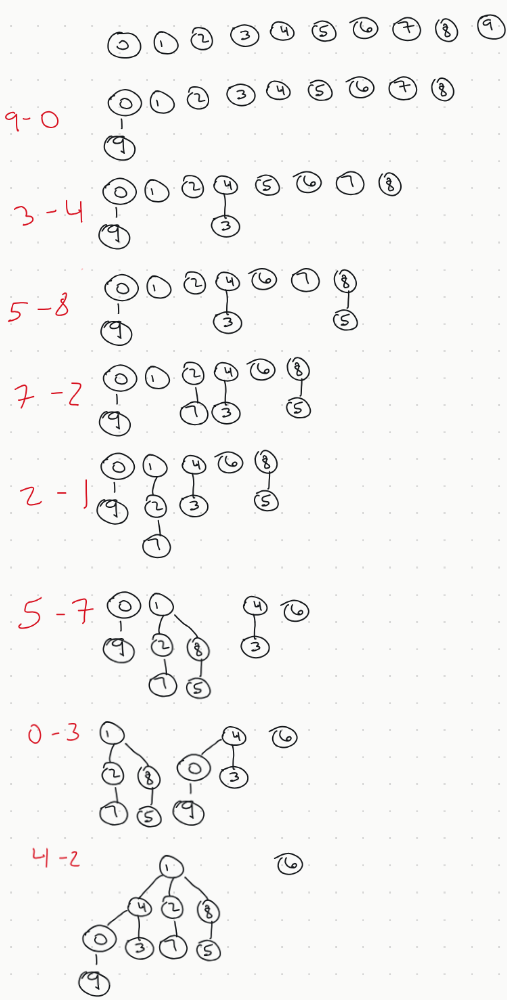
\includegraphics[width=0.5\textwidth]{exercise-02-quick-union-forest-of-trees}
			\caption{Forest of trees representation of \texttt{id[]} for quick-union in Exercise 2.}
			\label{ex-02}
		\end{figure}
	\end{sol}
	\begin{ex}{3}
		Do Exercise 1.5.1, but use weighted quick-union (page 228).
	\end{ex}
	\begin{sol}
		\begin{center}
			\begin{tabular}{cc|cccccccccc|c}
				\multicolumn{13}{c}{\texttt{id[]}}\\
				\texttt{p} & \texttt{q} & 0 & 1 & 2 & 3 & 4 & 5 & 6 & 7 & 8 & 9 & Array Accesses\\
				\hline
				9  & 0  & {\color{green} 0} & 1 & 2 & 3 & 4 & 5 & 6 & 7 & 8 & {\color{green} 9} & {}\\
				{} & {} & {\color{red} 9} & 1 & 2 & 3 & 4 & 5 & 6 & 7 & 8 & 9 & {}\\
				
				3  & 4  & 9 & 1 & 2 & {\color{green} 3} & {\color{green} 4} & 5 & 6 & 7 & 8 & 9 & {}\\
				{} & {} & 9 & 1 & 2 & 3 & {\color{red} 3} & 5 & 6 & 7 & 8 & 9 & {}\\
				
				5  & 8  & 9 & 1 & 2 & 3 & 3 & {\color{green} 5} & 6 & 7 & {\color{green} 8} & 9 & {}\\
				{} & {} & 9 & 1 & 2 & 3 & 3 & 5 & 6 & 7 & {\color{red} 5} & 9 & {}\\
				
				7  & 2 & 9 & 1 & {\color{green} 2} & 3 & 3 & 5 & 6 & {\color{green} 7} & {\color{red} 5} & 9 & {}\\
				{} & {} & 9 & 1 & {\color{red} 7} & 3 & 3 & 5 & 6 & 7 & {\color{red} 5} & 9 & {}\\
				
				2  & 1 & 9 & {\color{green}1} & {\color{green} 7} & 3 & 3 & 5 & 6 & {\color{green} 7} & 5 & 9 & {}\\
				{} & {} & 9 & {\color{red}7} & 7 & 3 & 3 & 5 & 6 & 7 & 5 & 9 & {}\\
				
				5  & 7 & 9 & {\color{green} 7} & {\color{green} 7} & 3 & 3 & {\color{green} 5} & 6 & {\color{green} 7} & {\color{green}5} & 9 & {}\\
				{} & {} & 9 & 7 & 7 & 3 & 3 & {\color{red} 7} & 6 & {\color{green} 7} & 5 & 9 & {}\\
				
				0  & 3  & {\color{green} 9} & 7 & 7 & {\color{green}3} & {\color{green}3} & 7 & 6 & 7 & 5 & {\color{green}9} & {}\\
				{} & {} & 9 & 7 & 7 & {\color{red}9} & 3 & 7 & 6 & 7 & 5 & 9 & {}\\
				
				4  & 2  & {\color{green}9} & {\color{green}7} & {\color{green}7} & {\color{green}9} & {\color{green}3} & {\color{green}7} & 6 & {\color{green}7} & {\color{green}5} & {\color{green}9} & {}\\
				{} & {} & 9 & 7 & 7 & 9 & 3 & 7 & 6 & 7 & 5 & {\color{red}7} & {}\\
			\end{tabular}
		\end{center}
		\begin{figure}
			\centering
			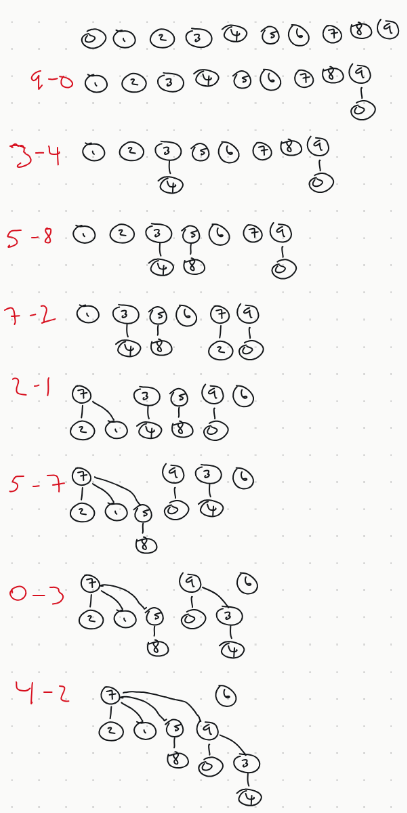
\includegraphics[width=0.5\textwidth]{exercise-03-weighted-quick-union-forest-of-trees}
			\caption{Forest of trees representation of \texttt{id[]} for quick-union in Exercise 2.}
			\label{ex-03}
		\end{figure}
		See Figure~\ref{ex-03}.
	\end{sol}
	\begin{ex}{7}
		Develop classes \texttt{QuickUnionUF} and \texttt{QuickFindUF} that implement quick-union
		and quick-find, respectively.
	\end{ex}
	\begin{sol}
		See the \texttt{com.segarciat.algs.ch1.sec5.ex07} package.
	\end{sol}
	\pagebreak
	\printbibliography
\end{document}